% Use only LaTeX2e, calling the article.cls class and 12-point type.

\documentclass[12pt]{article}

% Users of the {thebibliography} environment or BibTeX should use the
% scicite.sty package, downloadable from *Science* at
% http://www.sciencemag.org/authors/preparing-manuscripts-using-latex 
% This package should properly format in-text
% reference calls and reference-list numbers.

\usepackage{scicite}

\usepackage{times}
\usepackage{amsmath, amssymb}

% The preamble here sets up a lot of new/revised commands and
% environments.  It's annoying, but please do *not* try to strip these
% out into a separate .sty file (which could lead to the loss of some
% information when we convert the file to other formats).  Instead, keep
% them in the preamble of your main LaTeX source file.


%%%%%% taken from papaja-created ver
\usepackage{csquotes}
\usepackage{graphicx}
  \usepackage[unicode=true]{hyperref}
\usepackage{threeparttablex}            % Lets threeparttable work with longtable
  
% The following parameters seem to provide a reasonable page setup.

\topmargin 0.0cm
\oddsidemargin 0.2cm
\textwidth 16cm 
\textheight 21cm
\footskip 1.0cm


%The next command sets up an environment for the abstract to your paper.

\newenvironment{sciabstract}{%
\begin{quote} \bf}
{\end{quote}}


%EY: to add S to figure number in supplementary materials
\newcommand{\beginsupplement}{%
        \setcounter{table}{0}
        \renewcommand{\thetable}{S\arabic{table}}%
        \setcounter{figure}{0}
        \renewcommand{\thefigure}{S\arabic{figure}}%
     }

%EY: color for comments     
\usepackage[usenames, dvipsnames]{color}

\definecolor{Red}{RGB}{255,0,0}
\definecolor{Green}{RGB}{10,200,100}
\definecolor{Blue}{RGB}{10,100,200}
\definecolor{Orange}{RGB}{255,153,0}

\newcommand{\ejy}[1]{\textcolor{Red}{[ejy: #1]}}  
\newcommand{\ndg}[1]{\textcolor{Green}{[ndg: #1]}}  
\newcommand{\mht}[1]{\textcolor{Blue}{[mht: #1]}}  
\newcommand{\mcf}[1]{\textcolor{Orange}{[mcf: #1]}}

%EY: add packages
 \usepackage{lscape}
 \usepackage{array, booktabs, makecell}
 \usepackage{siunitx, mhchem}


% Include your paper's title here

\title{Polite speech emerges from competing pressures to be (and look)
informative and kind} 


% Place the author information here.  Please hand-code the contact
% information and notecalls; do *not* use \footnote commands.  Let the
% author contact information appear immediately below the author names
% as shown.  We would also prefer that you don't change the type-size
% settings shown here.

\author
%{Erica J. Yoon,$^{1\ast}$ Michael Henry Tessler,$^{1\ast}$ Noah D. Goodman,$^{1}$ Michael C. Frank$^{1}$\\
%\\
%\normalsize{$^{1}$Department of Psychology, Stanford University}\\
%\\
%\normalsize{$^\ast$These authors contributed equally to this work.}
%
%}
{Erica J. Yoon,$^{1\ast\dagger}$ Michael Henry Tessler,$^{1\ast}$ Noah D. Goodman,$^{1}$ Michael C. Frank$^{1}$\\
\\
\normalsize{$^{1}$Department of Psychology, Stanford University,}\\
\normalsize{450 Serra Mall, Stanford, CA 94305.}
\\
\normalsize{$^\ast$These authors contributed equally to this work.}
\\
\normalsize{$^\dagger$To whom correspondence should be addressed; E-mail: ejyoon@stanford.edu.}
}

% Include the date command, but leave its argument blank.

\date{}



%%%%%%%%%%%%%%%%% END OF PREAMBLE %%%%%%%%%%%%%%%%



\begin{document} 

% Double-space the manuscript.

\baselineskip24pt

% Make the title.

\maketitle 



% Place your abstract within the special {sciabstract} environment.

\begin{sciabstract}
Being polite, or conveying information in a false or indirect manner in
deference to someone else's feelings, seemingly contradicts an important
goal of a cooperative speaker: information transfer. In this work, we
show that polite speech emerges from a set of competing goals: to be
informative, to be kind, and to \emph{appear} helpful or kind. We
formalize this tradeoff between speaker's competing goals using a
utility-theoretic model, and show the model is able to predict people's
polite speech production judgments. Our extension of formal theories of
language to account for speakers' social goals represents an advance in
understanding of human language use.
\end{sciabstract}

% In setting up this template for *Science* papers, we've used both
% the \section* command and the \paragraph* command for topical
% divisions.  Which you use will of course depend on the type of paper
% you're writing.  Review Articles tend to have displayed headings, for
% which \section* is more appropriate; Research Articles, when they have
% formal topical divisions at all, tend to signal them with bold text
% that runs into the paragraph, for which \paragraph* is the right
% choice.  Either way, use the asterisk (*) modifier, as shown, to
% suppress numbering.

%%%%%%%%%%%%%%%%%%
%%%%% Introduction %%%%%%%
%%%%%%%%%%%%%%%%%%

We don't always say what we're thinking. Although \enquote{close the
window!} could be sufficient, we say \enquote{can you please\ldots{}?}
or \enquote{would you mind\ldots{}?} Rather than telling an
uncomfortable truth, we lie (\enquote{Your dress looks great!}) and
prevaricate (\enquote{Your poem was so appropriate to the occasion}).
Such utterances are puzzling for standard views of language use, which
see communication as the transfer of information from a sender to a
receiver \cite{buhler1934, shannon1948, jakobson1960, frank2012}. Under
information-based views, the transfer ought to be efficient and
accurate: The speaker should choose a succinct utterance  to convey
what the speaker knows \cite{grice1975, searle1975},
and the information transferred should be accurate and truthful 
to the extent of the speaker's knowledge. Polite speech --
like the examples above -- violates these basic expectations about the
nature of communication: It is typically inefficient and
underinformative, and sometimes even outright false. So why are we
polite?

Theories of politeness explain deviations from optimal information
transfer in language by assuming that speakers take into account social,
as well as informational, concerns. These concerns are sometimes
expressed as sets of polite maxims \cite{leech1983} or social norms \cite{ide1989}, 
but the most influential account of politeness relies on the
notion of \enquote{face} to motivate deviations \cite{brown1987, goffman1967}. 
On this theory, interactants seek to be liked,
approved, and related to (\enquote{positive face}) as well as maintain
their freedom to act (\enquote{negative face}).
Both inefficient indirect speech and untruthful lies in communication
are then the result of speakers' strategic choices relative to possible
face threats.

The face-based framework for polite language use provides an intuitive
and appealing explanation of many types of polite speech, but it does
not precisely define how competing communicative goals trade off with
one another. For example, it is unclear when the desire to save face
will motivate statements that are outright false (\enquote{Your cake is
delicious!}) versus indirect (\enquote{It could use a bit of salt}), and
when face-saving should be prioritized over other concerns (e.g.,
helpful information transfer).\\
Further, presentational goals related to face have not been formally
addressed: Speakers may choose particular strategies not only to
preserve the listener's face genuinely, but also to be \emph{seen} as
doing so, hence appearing to be considerate and socially apt and saving
their own face.

%%%%%%%%%%%%%%%%%%
%%%%%% Model %%%%%%%
%%%%%%%%%%%%%%%%%%

To address these challenges, we develop a utility-theoretic model to
quantify tradeoffs between different goals that a polite speaker may
have. In our model, speakers attempt to maximize a set of competing
utilities: an informational utility, derived via classical, effective
information transmission; a social utility, derived by being kind and
saving the listener's face; and a self-presentational utility, derived
by appearing in a particular way to save the speaker's own face.
Speakers then choose between different utterances on the basis of their
expected utility.

The utilities are weighed within a Rational Speech Act (RSA) model that
takes a probabilistic approach to pragmatic reasoning in language \cite{frank2012, goodman2016}: 
Speakers are modeled as agents
who choose utterances by reasoning about their effects on a listener
relative to their cost, while listeners are modeled as inferring
interpretations by reasoning about speakers and their goals. This class
of models has been effective in understanding a wide variety of complex
linguistic behaviors \cite{lassiter2017adjectival, kao2014, kao2015}, and, 
more broadly, the idea that human social cognition can
be approximated via reasoning about others as rational agents who act to
maximize their subjective utility \cite{baker2009action}, a
hypothesis which has found support in a wide variety of work with both
adults and children \cite{jara2016naive, liu2017ten}.

%\begin{figure}
%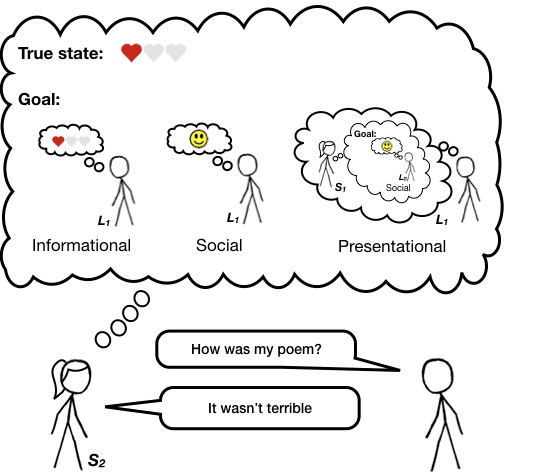
\includegraphics[width=6.23in]{fig/model} \caption{Diagram of the model: The pragmatic speaker observes the true state and determines her goal between three utilities (informational, social, and presentational), and produces an utterance.}\label{fig:model}
%\end{figure}


\begin{figure}
\centering
  \makebox[\textwidth]{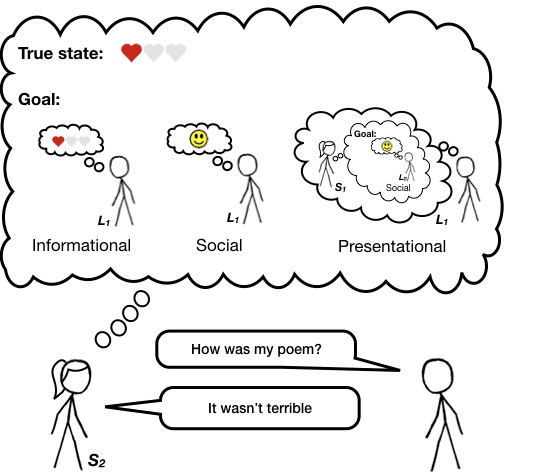
\includegraphics[width=0.8\textwidth]{fig/model}}
\caption{\label{fig:model}Diagram of the model: The pragmatic speaker observes the true state and determines her goal between three utilities (informational, social, and presentational), and produces an utterance.
}
\end{figure}


RSA models are defined recursively such that speakers reason about
listeners, and vice versa. By convention this recursion is indexed such
that a pragmatic listener \(L_1\) reasons about what intended meaning
and goals would have led a speaker \(S_1\) to produce a particular
utterance. Then \(S_1\) reasons about a \enquote{literal listener}
\(L_0\), modeled as attending only to the literal meanings of words
(rather than their pragmatic implications), and hence grounds the
recursion. The target of our current work is a model of a polite speaker
\(S_2\): \(S_2\) reasons about what utterance to say to \(L_1\) by
considering the set of utilities described above (Figure
@ref(fig:model)).

We evaluate our model by predicting human utterance choices in
situations where polite language use is expected. Imagine Bob recited
his poem and asks Ann how well he did. Ann (\(S_2\)) produces an
utterance \(w\) based on the true state of the world \(s\) (i.e., the
rating truly deserved by Bob's recital) and a set of goal weights
\(\hat{\phi}\), that determines how much Ann prioritizes each goal.
Ann's production decision is softmax, which interpolates between
maximizing and probability matching (\(\lambda_{S_2}\); \cite{goodman2013}):

\[P_{S_2}(w | s, \hat{\phi}) \propto \exp(\lambda_{S_2} \cdot \mathop{\mathbb{E}}[U_{total}(w; s; \hat{\phi})])\].

What goals must the speaker consider to arrive at a polite utterance? We
consider three utilities: informational, social, and presentational. The
total utility of an utterance is the weighted combination of the three
utilities minus the utterance cost \(C(w)\):

\[U_{total}(w; s; \hat{\phi}) = \phi_{inf} \cdot U_{inf}(w; s) + \phi_{soc} \cdot U_{soc}(w; s) + \phi_{pres} \cdot U_{pres}(w; s) - C(w)\].

The first utility term is a standard \emph{informational utility}
(\(U_{inf}\)), which represents the speaker's desire to be epistemically
helpful. The informational utility captures the amount of information a
literal listener (\(L_0\)) would still not know about the world state
after hearing the speaker's utterance:
\(U_{inf}(w) = \ln(P_{L_1}(s | w))\).

Second, we define the \emph{social utility} (\(U_{soc}\)) as the value
\(V(s)\), or expected subjective utility, to the listener of the state
inferred given the utterance:
\(U_{soc}(w) = \mathbb{E}_{P_{L_1}(s \mid w)}[V(s)]\). This value
captures the idea that listeners want to hear that they are in a good
state of the world (e.g., Bob would prefer that his poem was good).

If listeners try to infer the goals that a speaker is entertaining
(e.g., social vs.~informational), speakers may choose utterances in
order to convey that they had certain goals in mind. The third and the
most novel component of our model, \emph{presentational utility}
(\(U_{pres}\)), captures the extent to which the speaker appears to the
listener to have a particular goal in mind (e.g., to be kind). Formally,

\[U_{pres}(w) = \ln(P_{L_1}(\phi_{S_1} \mid w)) = \ln \int_s P_{L_1}(s, \phi_{S_1} \mid w)\].

The speaker considers the beliefs of listener \(L_1\), who hears an
utterance and jointly infers both the speaker's utilities and the true
state of the world:

\[P_{L_1}(s, \hat{\phi} | w) \propto P_{S_1}(w | s, \hat{\phi}) \cdot P(s) \cdot p(\hat{\phi})\].

This presentational utility is higher-order in that it can only be
defined for a speaker thinking about a listener who evaluates a speaker.
(i.e., it can be defined for \(S_2\), but not \(S_1\).)

Finally, more complex utterances incur a greater cost, \(C(w)\) --
capturing the general pressure towards economy in speech. In our work,
utterances with negation (e.g., \enquote{not terrible}) are assumed to
be slightly costlier than their equivalents with no negation.

Intuitively, if Bob's performance was good, Ann's utilities align toward
a positive utterance. By saying \enquote{{[}Your poem{]} was amazing,}
Ann is simultaneously being truthful, kind, and appearing both truthful
and kind. If Bob's performance was poor, however, Ann is in a bind: Ann
could be kind and say \enquote{It was great}, but at the cost of
conveying the wrong information to Bob if he believes her to be
truthful. Or, worse yet, Bob could infer Ann is \enquote{just being
nice}, and think of her as a dishonest, unhelpful speaker.
Alternatively, she could say the truth (\enquote{It was bad}), but then
Bob would think Ann didn't care about him. What is a socially-aware
speaker to do? Our model predicts that indirect speech -- like
\enquote{It wasn't bad} -- helps navigate Ann's dilemma. It conveys some
true information (e.g., literally it wasn't the worst it could have
been) while being sufficiently open-ended to spare Bob's feelings.
Further, by incurring the slightly higher cost involved in producing
negation, Bob could reason that Ann had reasons for not saying a simpler
alternative like \enquote{It was good} and that she must have taken his
feelings into account in her utterance.

%%%%%%%%%%%%%%%%%%
%%%%% Human data %%%%%%%
%%%%%%%%%%%%%%%%%%

We tested our model in an online experiment (\emph{N} = 202).
Participants read scenarios with information about the speaker's
feelings toward some performance or product (e.g., poem recital;
\emph{true state}), on a scale from zero to three hearts. We manipulated
the speaker's \emph{goal} across trials: to be \emph{informative}
(\enquote{give accurate and informative feedback}); to be \emph{kind}
(\enquote{make the listener feel good}); or to be \emph{both}
informative and kind simultaneously. We hypothesized that each of the
three goals will represent a tradeoff between the three utilities in our
model (see Supplementary Materials). In a single trial, each scenario
was followed by a question asking for the most likely utterance by Ann.
Participants selected one of eight possible utterances, by choosing
between \emph{It was} vs. \emph{It wasn't} and then among
\emph{terrible}, \emph{bad}, \emph{good}, and \emph{amazing.}

%%%%%%%%%%%%%%%%%%
%%%%% Results %%%%%%%
%%%%%%%%%%%%%%%%%%

\begin{figure}
\centering
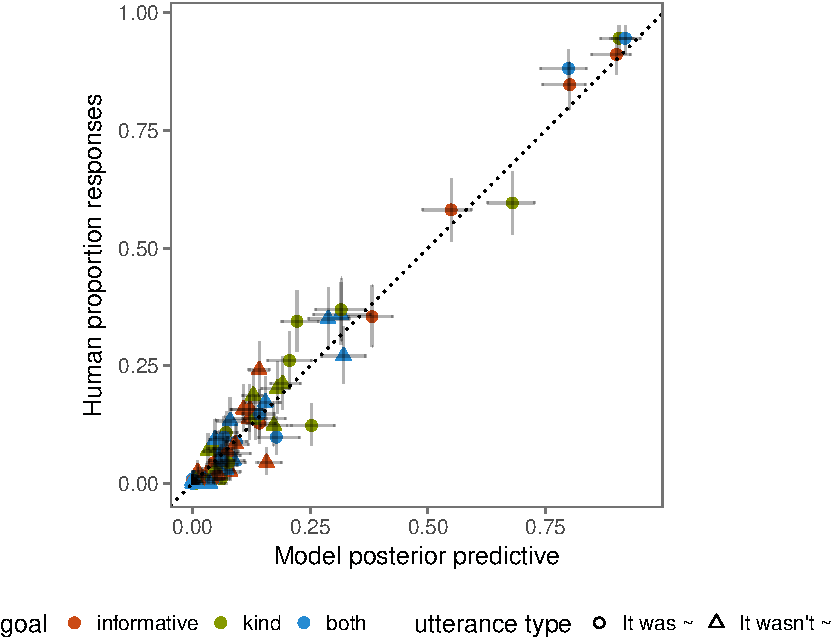
\includegraphics{polite_manuscript_files/figure-latex/variance-1.pdf}
\caption{\label{fig:variance}Full distribution of human responses vs.~model
predictions. Error bars represent 95\% confidence intervals for the data
(vertical) and 95\% highest density intervals for the model
(horizontal).}
\end{figure}

Our primary behavioral hypothesis was that speakers describing bad
states (e.g., Bob's performance deserved 0 heart) with goals to be both
informative and kind would produce more indirect, negative utterances
(e.g., \enquote{It wasn't terrible}). Such indirect speech acts serve to
save the listener's face while also conveying a vague estimate of the
true state. This prediction was confirmed: a Bayesian mixed-effects
model predicting negation as a function of true state and goal yielded
an interaction such that a speaker with both goals to be informative and
kind produced more negation in worse states compared to a speaker with
only the goal to be informative (\emph{M} = -1.33, {[}-1.69, -0.98{]})
and goal to be kind (\emph{M} = -0.50, {[}-0.92, -0.07{]}).

To connect these behavioral data more directly to our model, we
separately obtained literal meaning judgments about the utterances and
incorporated them into our model's predictions. Using an independent
sample (\emph{N}=51), we measured judgments of how well different
utterances apply to each of the levels on the heart scale (e.g., to what
extent is \enquote{terrible} true of 2 out of 3 hearts?). These
measurements were used to approximate the semantics of the words as
interpreted by the literal listener \(L_0\). 
Then we used a Bayesian analytic technique \cite{lee2014} 
to infer the parameters of
the model (e.g., the speaker's utility weights in each goal condition;
see Supplementary Materials).

\begin{figure}
\centering
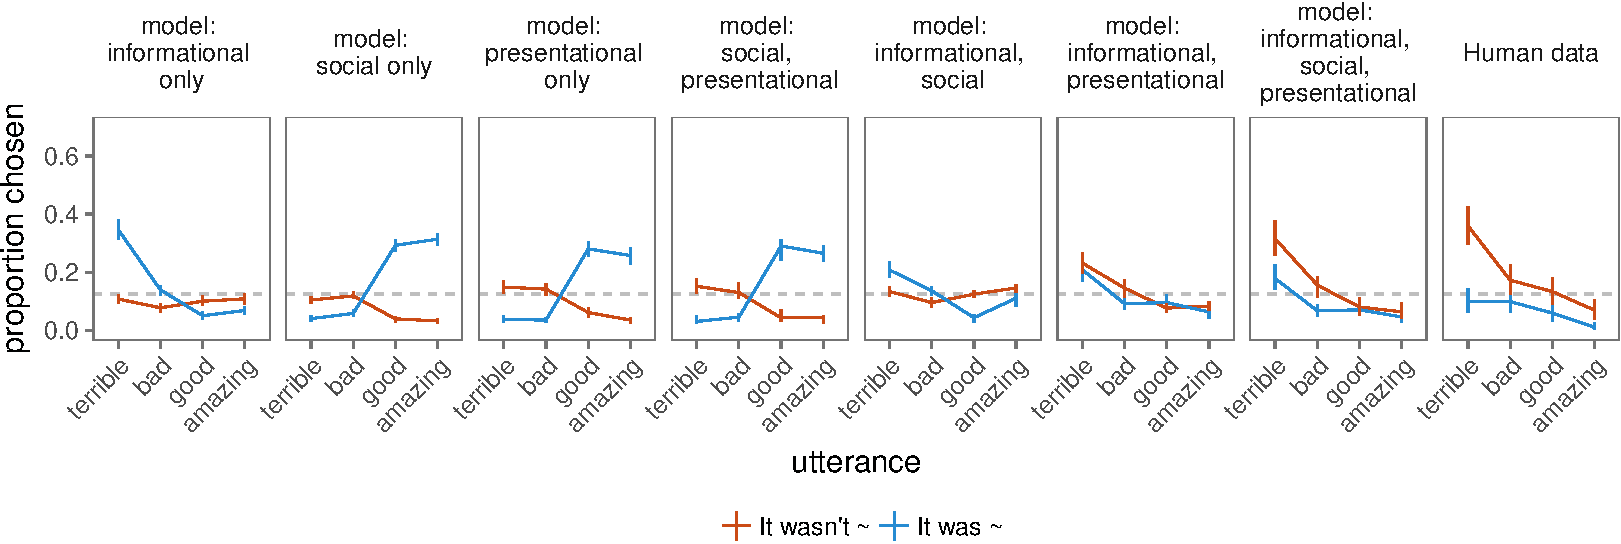
\includegraphics[width=\textwidth]{polite_manuscript_files/figure-latex/comparison-1.pdf}
\caption{\label{fig:comparison}Comparison of predictions for proportion of
utterances chosen by pragmatic speaker from possible model variants
(left) and human data (rightmost) for average proportion of negation
produced among all utterances, given true state of 0 heart (on a scale
of 0 to 3) and speaker with both goals. Gray dotted line indicates
chance level at 12.5\%.}
\end{figure}

\begin{table}[tbp]
\begin{center}
\begin{threeparttable}
\caption{\label{tab:comparisonTable}Comparison of variance explained for each model variant and log Bayes Factors quantifying evidence in favor of the full model, in comparison to each of the alternatives.}
\begin{tabular}{lll}
\toprule
Model & \multicolumn{1}{c}{Variance 
explained} & \multicolumn{1}{c}{log BF}\\
\midrule
model: 
informative only & 0.83 & 274.89\\
model: 
social only & 0.22 & 885.52\\
model: 
presentational 
only & 0.23 & 873.83\\
model: 
social, 
presentational & 0.23 & 864.00\\
model: 
informative, 
social & 0.92 & 25.06\\
model: 
informative, 
presentational & 0.96 & 11.14\\
model: 
informative, 
social, 
presentational & 0.97 & 1.00\\
\bottomrule
\end{tabular}
\end{threeparttable}
\end{center}
\end{table}

Predictions from the full polite speaker model showed a very strong fit
to participants' utterance choices (\(r^2\)(96) = 0.97; Figure
\ref{fig:variance}). We also compared the predictions of our model with
its variants containing subsets of the three utilities in the full model
(Figure 3). Both the variance explained and the marginal likelihood of
the observed data were the highest for the full model (see Table
\ref{tab:comparisonTable} and Figure \ref{fig:comparison}). In
particular, only the full model captured the participants' preference
for negation in the condition in which the speaker had both goals to be
informative and kind about truly bad states, as hypothesized. Thus, all
three utilities -- informational, social, and presentational -- were
required to fully explain participants' choices.

%%%%%%%%%%%%%%%%%%
%%%%% Implications %%%%%%%
%%%%%%%%%%%%%%%%%%

To better measure choice behavior, our experiment abstracted away from
natural interactions in a number of ways. Real-life Anns will have
access to a potentially infinite range of utterances to manage the same
tradeoff (\enquote{It's hard to write a good poem}, \enquote{That
metaphor in the second stanza was so relatable!}). Under our framework,
each utterance will have strengths and weaknesses relative to the
speaker's goals, though computation in an unbounded model presents
technical challenges (see \cite{goodman2016}).

Managing listeners' inferences is a fundamental task for a socially
conscious speaker. Following Brown and Levinson (1987), cross-cultural
differences in politeness could be a product of different weightings
within the same utility structure. It is also possible, however, that
culture affects the value function \(V\) that maps states of the world
onto subjective values for the listener (e.g., the mapping from states
to utilities may be more complex than we have considered). Our formal
modeling approach with systematic behavior measurements provides an
avenue towards understanding the vast range of politeness practices
found across languages.

Our work extends previous models of language beyond standard
informational utilities to address social and self-presentational
concerns. Previous theories of language use have not explained how
informational versus social concerns trade off to inform the speaker's
utterance choices. Thus, this work represents a key theoretical advance
exploring how informational cooperativity interacts with other social
goals. The current work also opens up important communicative behaviors
to formal modeling. Politeness is just one of the ways that language use
deviates from pure information transfer; When we flirt, insult, boast,
and empathize, we balance information transmission with the goal to
affect others' feelings or present particular views of ourselves. A
similar utility structure to our model could give insights into these
speech acts as well as a wide range of behaviors that can be modeled as
utility-driven inference in a social context \cite{baker2017rational, hamlin2013mentalistic} 
where agents need to take into account concerns about both self
and others.

In sum, this work takes a concrete step toward quantitative models of
the nuances of human speech. And it moves us closer to courteous
computation -- to computers that communicate with tact.


% Your references go at the end of the main text, and before the
% figures.  For this document we've used BibTeX, the .bib file
% scibib.bib, and the .bst file Science.bst.  The package scicite.sty
% was included to format the reference numbers according to *Science*
% style.

%BibTeX users: After compilation, comment out the following two lines and paste in
% the generated .bbl file. 

\bibliography{politeness}

\bibliographystyle{Science}





\section*{Acknowledgments}
\emph{Funding}: This work was supported by NSERC PGS Doctoral scholarship
PGSD3-454094-2014 to EJY, NSF Graduate Research Fellowship DGE-114747 to
MHT, ONR grant N00014-13-1-0788 to NDG, and NSF grant BCS 1456077 to
MCF. 
\emph{Author contributions}: E.J.Y., M.H.T., N.D.G., and M.C.F. designed research; 
E.J.Y. and M.H.T. performed research; E.J.Y. and M.H.T. analyzed data; and E.J.Y., M.H.T., N.D.G., and M.C.F. wrote the paper.
\emph{Competing interests}: The authors declare no conflict of interest.
\emph{Data and materials availability}: Our pre-registered model,
hypothesis, and procedure, as well as all of our data and analyses are available at
\url{https://github.com/ejyoon/polite_speaker}.

%Here you should list the contents of your Supplementary Materials -- below is an example. 
%You should include a list of Supplementary figures, Tables, and any references that appear only in the SM. 
%Note that the reference numbering continues from the main text to the SM.
% In the example below, Refs. 4-10 were cited only in the SM.     

\section*{Supplementary materials}

\subsection*{Materials and Methods}\label{materials-and-methods}

\subsubsection*{Literal semantic task}\label{literal-semantic-task}

We probed judgments of literal meanings of the target words assumed by
our model and used in our main experiment. 51 participants with IP
addresses in the United States were recruited on Amazon's Mechanical
Turk. We used thirteen different context items in which a speaker
evaluated a performance of some kind. For example, in one of the
contexts, Ann saw a presentation, and Ann's feelings toward the
presentation (true state) were shown on a scale from zero to three
hearts (e.g., two out of three hearts filled in red color; see
Figure~\ref{fig:screenshot} for an example of the heart scale). The
question of interest was \enquote{Do you think Ann thought the
presentation was / wasn't X?} and participants responded by choosing
either \enquote{no} or \enquote{yes.} The target could be one of four
possible words: \emph{terrible}, \emph{bad}, \emph{good}, and
\emph{amazing}, giving rise to eight different possible utterances (with
negation or no negation). Each participant read 32 scenarios, depicting
every possible combination of states and utterances. The order of
context items was randomized, and there were a maximum of four repeats
of each context item per participant. For this and the speaker
production experiment, we analyzed the data by collapsing across context
items. For each utterance-state pair, we computed the posterior
distribution over the semantic weight (i.e., how consistent X utterance
is with Y state) assuming a uniform prior over the weight (i.e., a
standard Beta-Binomial model). Meanings of the words as judged by
participants were as one would expect (Figure ~\ref{fig:litsem}).

\subsubsection*{Speaker production task}\label{speaker-production-task}

202 participants with IP addresses in the United States were recruited
on Amazon's Mechanical Turk. As in the literal semantic task above, we
used scenarios in which a person (e.g., Bob) gave some performance and
asked for another person (e.g., Ann)'s opinion on the performance (see
Fig. 2). Additionally, we provided information on the speaker Ann's goal
-- to make Bob feel good, or to give as accurate and informative
feedback as possible, or both -- and the true state -- how Ann actually
felt about Bob's performance (e.g., two out of three hearts, on a scale
from zero to three hearts; Figure~\ref{fig:screenshot}). Each
participant read twelve scenarios, depicting every possible combination
of the three goals and four states. The order of context items was
randomized, and there were a maximum of two repeats of each context item
per participant. Each scenario was followed by a question that read,
\enquote{If Ann wanted to make Bob feel good but not necessarily give
informative feedback (or to give accurate and informative feedback but
not necessarily make Bob feel good, or BOTH make Bob feel good AND give
accurate and informative feedback), what would Ann be most likely to
say?} Participants indicated their answer by choosing one of the options
on the two dropdown menus, side-by-side, one for choosing between
\emph{It was} vs. \emph{It wasn't} and the other for choosing among
\emph{terrible}, \emph{bad}, \emph{good}, and \emph{amazing.}

\subsection*{Supplementary Text}\label{supplementary-text}

\subsubsection*{Data analysis}\label{data-analysis}

We used R (Version 3.4.3; R Core Team, 2017) and the R-packages
\emph{BayesFactor} (Version 0.9.12.2; Morey \& Rouder, 2015),
\emph{bindrcpp} (Version 0.2; Müller, 2017a), \emph{binom} (Version
1.1.1; Dorai-Raj, 2014), \emph{brms} (Version 2.0.1; Bürkner, 2017),
\emph{coda} (Version 0.19.1; Plummer, Best, Cowles, \& Vines, 2006),
\emph{directlabels} (Version 2017.3.31; Hocking, 2017), \emph{dplyr}
(Version 0.7.4; Wickham, Francois, Henry, \& Müller, 2017),
\emph{forcats} (Version 0.2.0; Wickham, 2017a), \emph{ggplot2} (Version
2.2.1; Wickham, 2009), \emph{ggthemes} (Version 3.4.0; Arnold, 2017),
\emph{gridExtra} (Version 2.3; Auguie, 2017), \emph{here} (Version 0.1;
Müller, 2017b), \emph{jsonlite} (Version 1.5; Ooms, 2014),
\emph{langcog} (Version 0.1.9001; Braginsky, Yurovsky, \& Frank, n.d.),
\emph{lme4} (Version 1.1.15; Bates, Mächler, Bolker, \& Walker, 2015),
\emph{magrittr} (Version 1.5; Bache \& Wickham, 2014), \emph{Matrix}
(Version 1.2.12; Bates \& Maechler, 2017), \emph{papaja} (Version
0.1.0.9655; Aust \& Barth, 2017), \emph{purrr} (Version 0.2.4; Henry \&
Wickham, 2017), \emph{RColorBrewer} (Version 1.1.2; Neuwirth, 2014),
\emph{Rcpp} (Eddelbuettel \& Balamuta, 2017; Version 0.12.14;
Eddelbuettel \& François, 2011), \emph{readr} (Version 1.1.1; Wickham,
Hester, \& Francois, 2017), \emph{rwebppl} (Version 0.1.97; Braginsky,
Tessler, \& Hawkins, n.d.), \emph{stringr} (Version 1.2.0; Wickham,
2017b), \emph{tibble} (Version 1.3.4; Müller \& Wickham, 2017),
\emph{tidyr} (Version 0.7.2; Wickham \& Henry, 2017), and
\emph{tidyverse} (Version 1.2.1; Wickham, 2017c) for all our analyses.


\setcounter{table}{0}    
\beginsupplement

\subsubsection*{Full statistics on human
data}\label{full-statistics-on-human-data}

\begin{table}[tbp]
\begin{center}
\begin{threeparttable}
\caption{\label{tab:brmTab}Predictor mean estimates with standard deviation and 95\% credible interval information for a Bayesian linear mixed-effects model predicting negation production based on true state and speaker goal (with both-goal as the reference level).}
\begin{tabular}{lllll}
\toprule
Predictor & \multicolumn{1}{c}{Mean} & \multicolumn{1}{c}{SD} & \multicolumn{1}{c}{95\% CI-Lower} & \multicolumn{1}{c}{95\% CI-Upper}\\
\midrule
Intercept & 0.88 & 0.13 & 0.63 & 1.12\\
True state & 2.18 & 0.17 & 1.86 & 2.53\\
Goal: Informative & 0.47 & 0.17 & 0.14 & 0.80\\
Goal: Social & 0.97 & 0.25 & 0.51 & 1.49\\
True state * Informative & -1.33 & 0.18 & -1.69 & -0.98\\
True state * Social & -0.50 & 0.22 & -0.92 & -0.07\\
\bottomrule
\end{tabular}
\end{threeparttable}
\end{center}
\end{table}

We used Bayesian linear mixed-effects models (\texttt{brms} package in
R; Bürkner, 2017) using crossed random effects of true state and goal
with maximal random effects structure (Barr, Levy, Scheepers, \& Tily,
2013).

\subsubsection*{Polite RSA model fitting and inferred
parameters}\label{polite-rsa-model-fitting-and-inferred-parameters}

\begin{table}[tbp]
\begin{center}
\begin{threeparttable}
\caption{\label{tab:phi}Inferred phi parameters from all model variants with more than one utility.}
\begin{tabular}{llllll}
\toprule
Model & \multicolumn{1}{c}{goal} & \multicolumn{1}{c}{$\phi_{inf}$} & \multicolumn{1}{c}{$\phi_{soc}$} & \multicolumn{1}{c}{$\phi_{pres}$} & \multicolumn{1}{c}{$\phi_{S_1}$}\\
\midrule
informative, social, presentational & both & 0.36 & 0.11 & 0.54 & 0.36\\
informative, social, presentational & informative & 0.36 & 0.02 & 0.62 & 0.49\\
informative, social, presentational & social & 0.25 & 0.31 & 0.44 & 0.37\\
informative, presentational & both & 0.64 & NA & 0.36 & 0.17\\
informative, presentational & informative & 0.77 & NA & 0.23 & 0.33\\
informative, presentational & social & 0.66 & NA & 0.34 & 0.04\\
informative, social & both & 0.54 & 0.46 & NA & NA\\
informative, social & informative & 0.82 & 0.18 & NA & NA\\
informative, social & social & 0.39 & 0.61 & NA & NA\\
social, presentational & both & NA & 0.38 & 0.62 & 0.55\\
social, presentational & informative & NA & 0.35 & 0.65 & 0.75\\
social, presentational & social & NA & 0.48 & 0.52 & 0.66\\
\bottomrule
\end{tabular}
\end{threeparttable}
\end{center}
\end{table}

\begin{table}[tbp]
\begin{center}
\begin{threeparttable}
\caption{\label{tab:otherParams}Inferred negation cost and speaker optimality parameters for all model variants.}
\begin{tabular}{lll}
\toprule
Model & \multicolumn{1}{c}{Cost of negation} & \multicolumn{1}{c}{Speaker optimality}\\
\midrule
informative only & 1.58 & 8.58\\
informative, presentational & 1.89 & 2.93\\
informative, social & 1.11 & 3.07\\
informative, social, presentational & 2.64 & 4.47\\
presentational only & 2.58 & 9.58\\
social only & 1.73 & 7.23\\
social, presentational & 2.49 & 5.29\\
\bottomrule
\end{tabular}
\end{threeparttable}
\end{center}
\end{table}

In the speaker production task, participants were told the speakers'
intentions (e.g., wanted to make Bob feel good). We assume that the
intention descriptions conveyed some mixture of weights \(\phi_{epi}\),
\(\phi_{soc}\), \(\phi_{pres}\), and \(\phi_{S_1}\) that the speaker was
using. We put uninformative priors on the unnormalized mixture weights
(\(\phi\) \textasciitilde{} \(Uniform(0,1)\)) separately for each goal
condition (\enquote{wanted to be X}; \emph{informative}, \emph{kind}, or
\emph{both}). In addition, the full model has two global parameters: the
speaker's soft-max parameter \(\lambda_{S_2}\) and soft-max paramater of
the hypothetical speaker that the pragmatic listener reasons about
\(\lambda_{S_1}\). \(\lambda_{S_1}\) was 1, and \(\lambda_{S_2}\) was
inferred from the data: We put a prior that was consistent with those
used for similar models in this model class: \(\lambda_{S_2}\)
\textasciitilde{} \(Uniform(0,20)\). Finally, we incorporate the literal
semantics data into the RSA model by maintaining uncertainty about the
semantic weight of utterance \(w\) for state \(s\), for each of the
states and utterances, and assuming a Beta-Binomial linking function
between these weights and the literal semantics data (see \emph{Literal
semantics task} above). We infer the posterior distribution over all of
the model parameters and generate model predictions based on this
posterior distribution using Bayesian data analysis (Lee \& Wagenmakers,
2014). We ran 4 MCMC chains for 80,000 iterations, discarding the first
40,000 for burnin. The inferred values of weight mixtures for each model
variant (with different \(\phi\) components) and other parameters are
shown in Table \ref{tab:phi} and Table \ref{tab:otherParams},
respectively.

\newpage

\subsection*{Figs. \ref{fig:screenshot} to \ref{fig:negation}}\label{supplemental-figures}

\setcounter{figure}{0}    
\beginsupplement

\begin{figure}[!h]
\centering
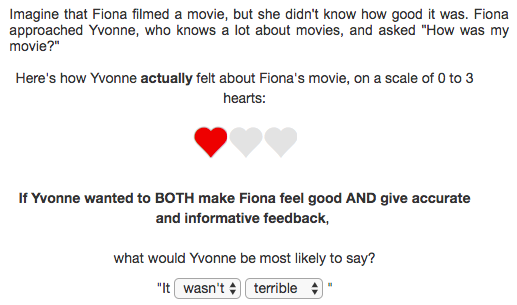
\includegraphics[width=3.98in]{fig/screenshot} \caption{Example of a trial in the speaker production task.}\label{fig:screenshot}
\end{figure}

\begin{figure}[!h]
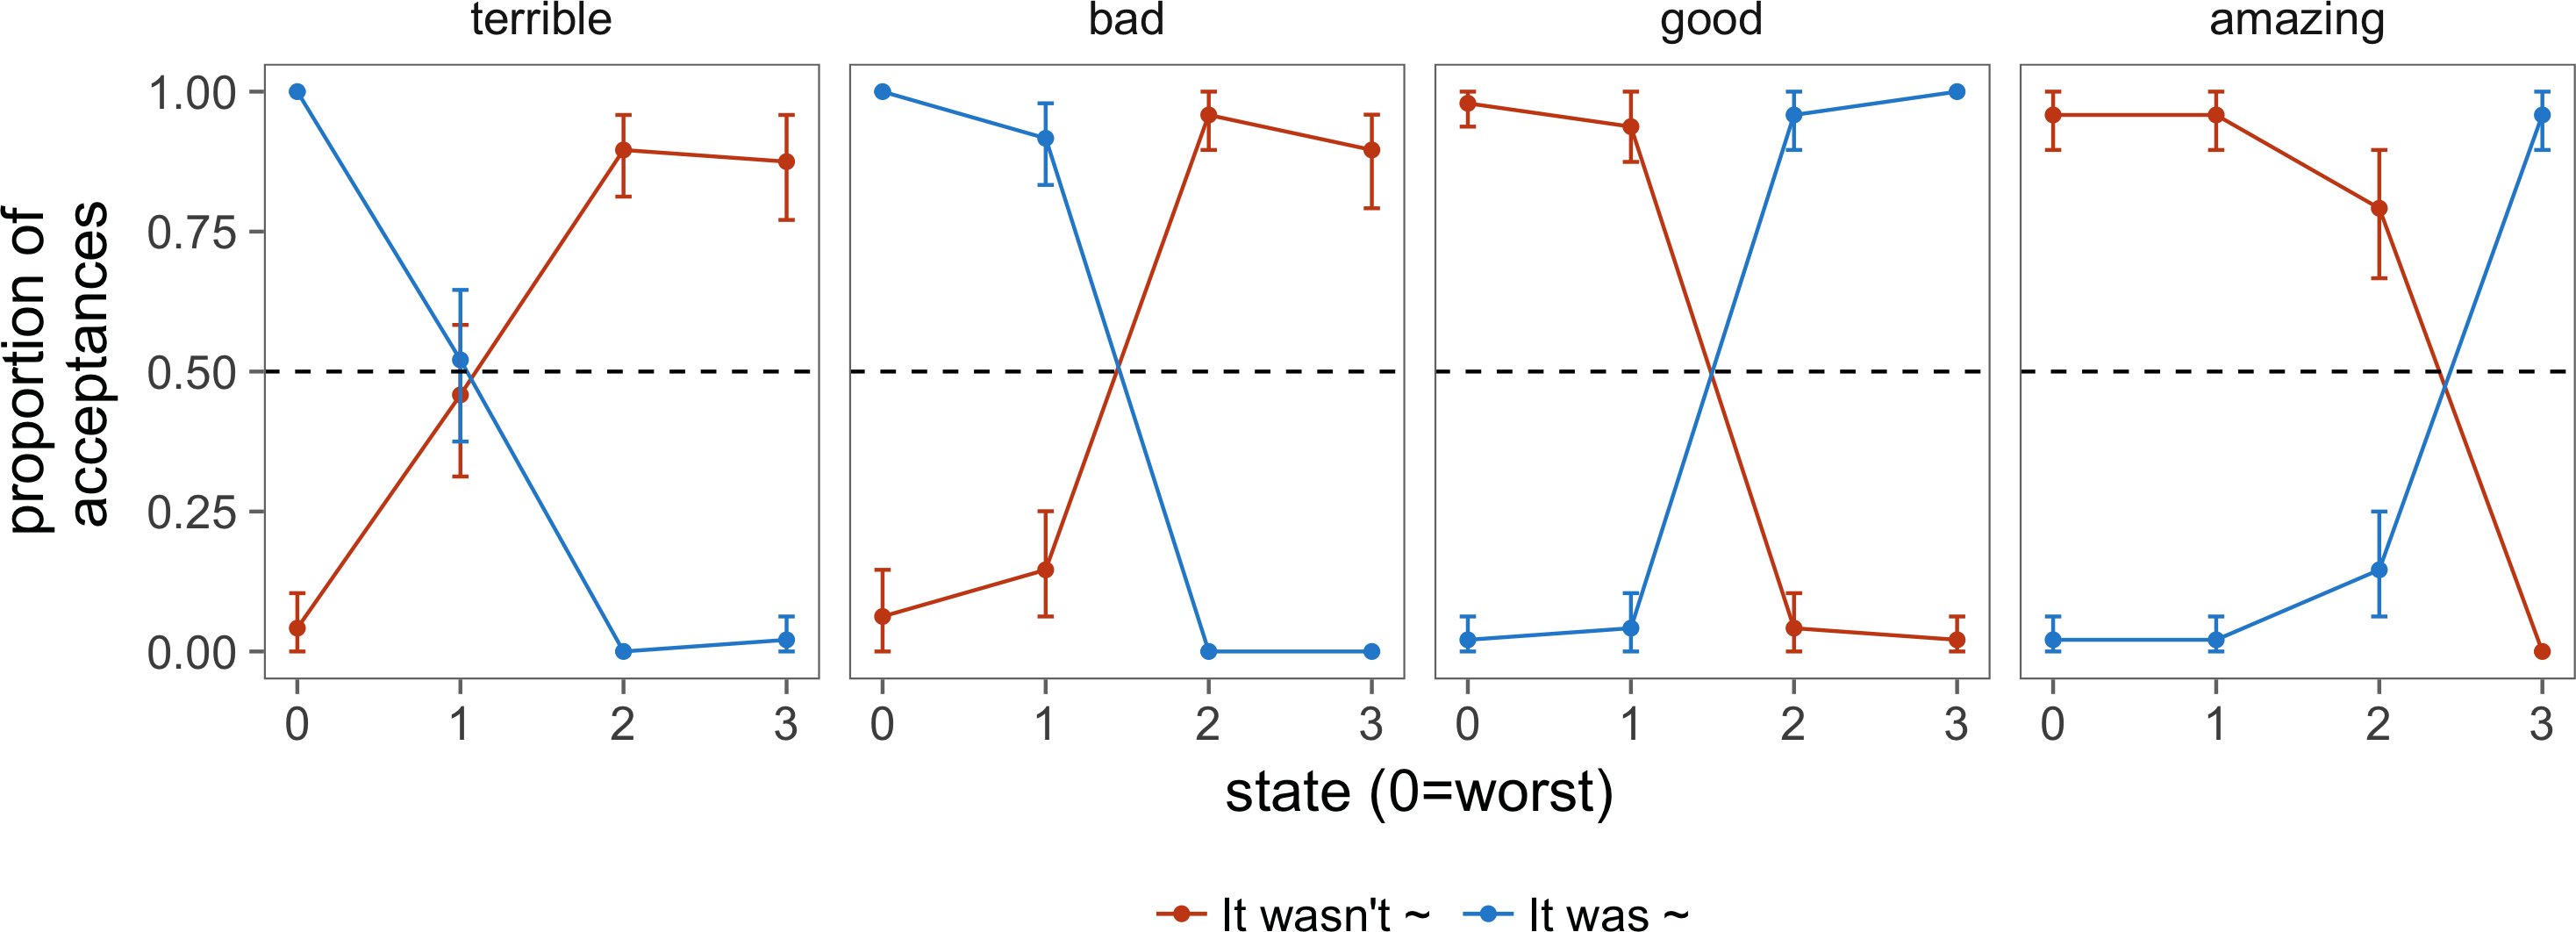
\includegraphics[width=\textwidth]{polite_manuscript_files/figure-latex/litsem-1} \caption{Semantic measurement results. Proportion of acceptances of utterance types (shown in different colors) combined with target words (shown in different facets) given the true state represented on a scale of hearts. Error bars represent 95\% confidence intervals.}\label{fig:litsem}
\end{figure}

\begin{figure}[!h]
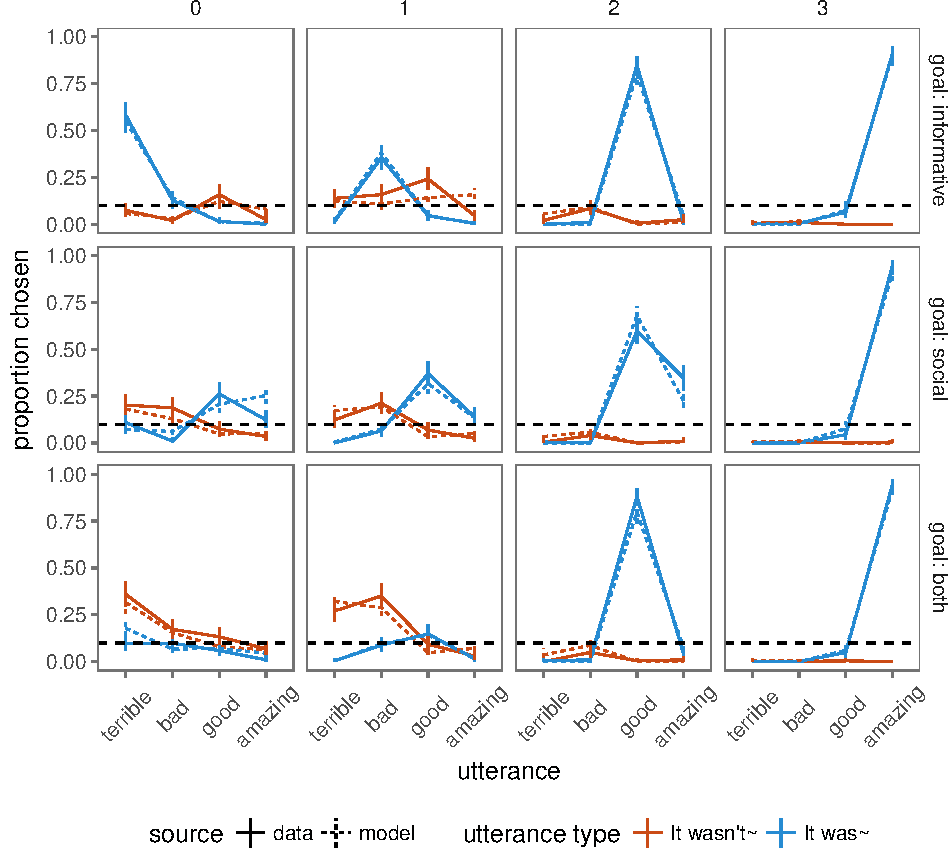
\includegraphics[width=\textwidth]{polite_manuscript_files/figure-latex/utterance-1} \caption{Experimental results (solid lines) and fitted predictions from the full model (dashed lines) for speaker production. Proportion of utterances chosen (utterance type – direct vs. indirect – in different colors and words shown on x-axis) given the true states (columns) and speaker goals (rows). Error bars represent 95\% confidence intervals for the data and 95\% highest density intervals for the model. Black dotted line represents the chance level.}\label{fig:utterance}
\end{figure}

\begin{figure}[!h]
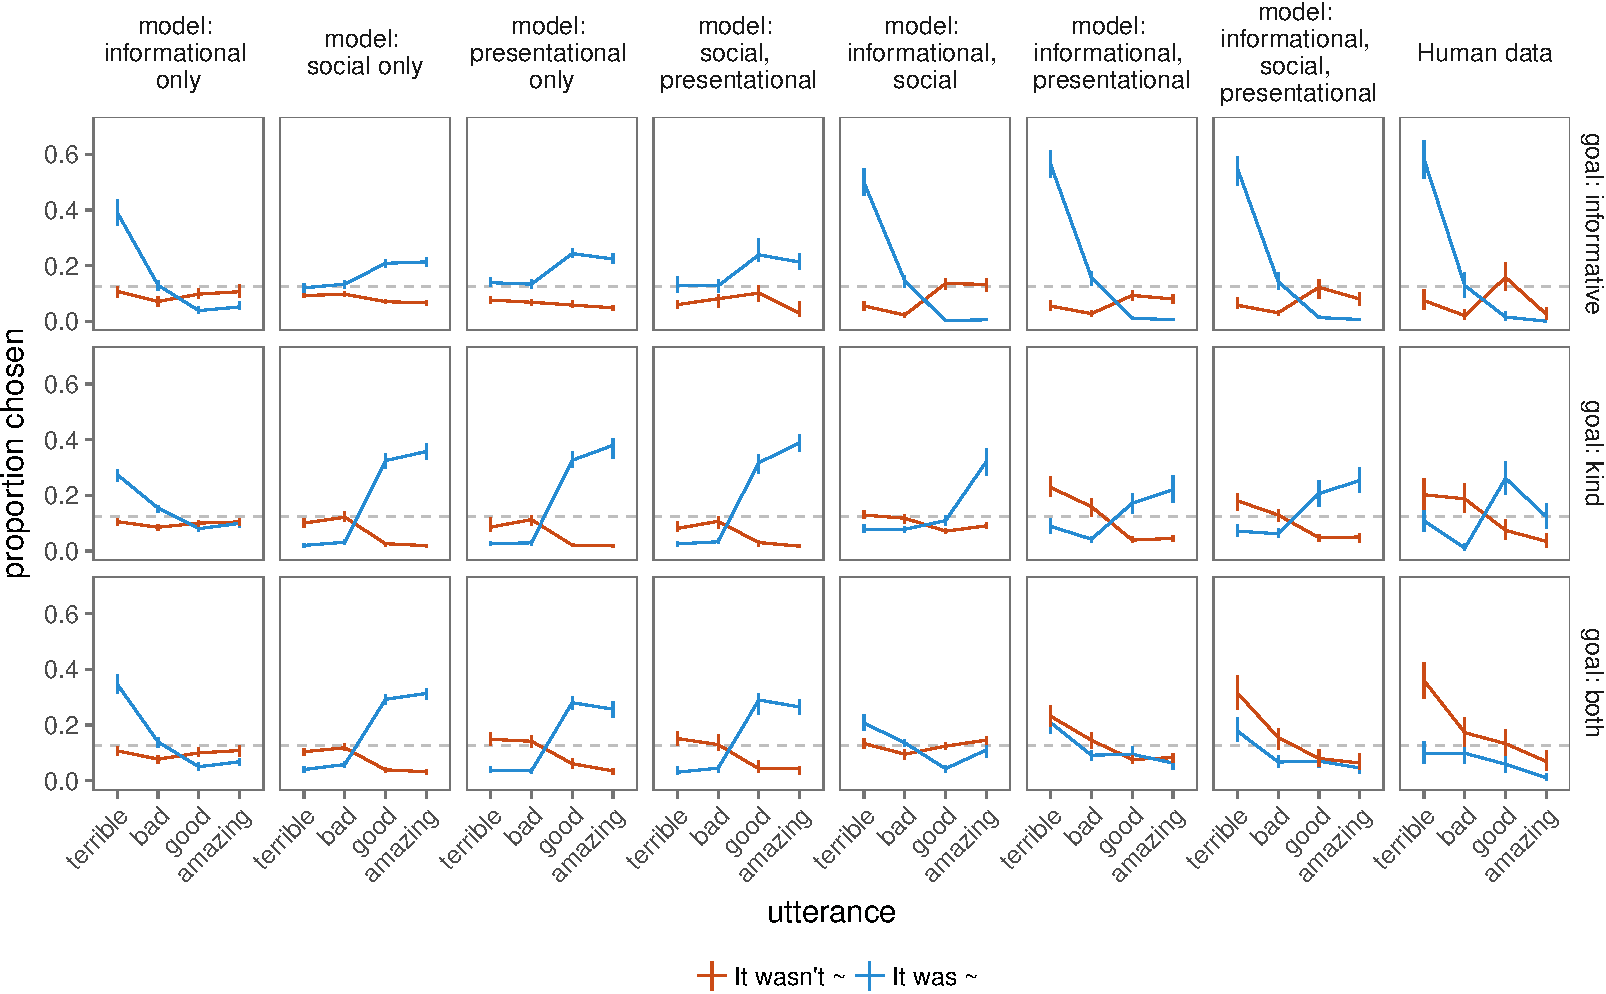
\includegraphics[width=\textwidth]{polite_manuscript_files/figure-latex/comparisonAll-1} \caption{Comparison of predictions for proportion of utterances chosen by pragmatic speaker from possible model variants (left) and human data (rightmost) for average proportion of negation produced among all utterances, given true state of 0 heart and speaker with a goal to be informative (top), kind (middle), or both (bottom). Gray dotted line indicates chance level at 12.5\%.}\label{fig:comparisonAll}
\end{figure}

\begin{figure}[!h]
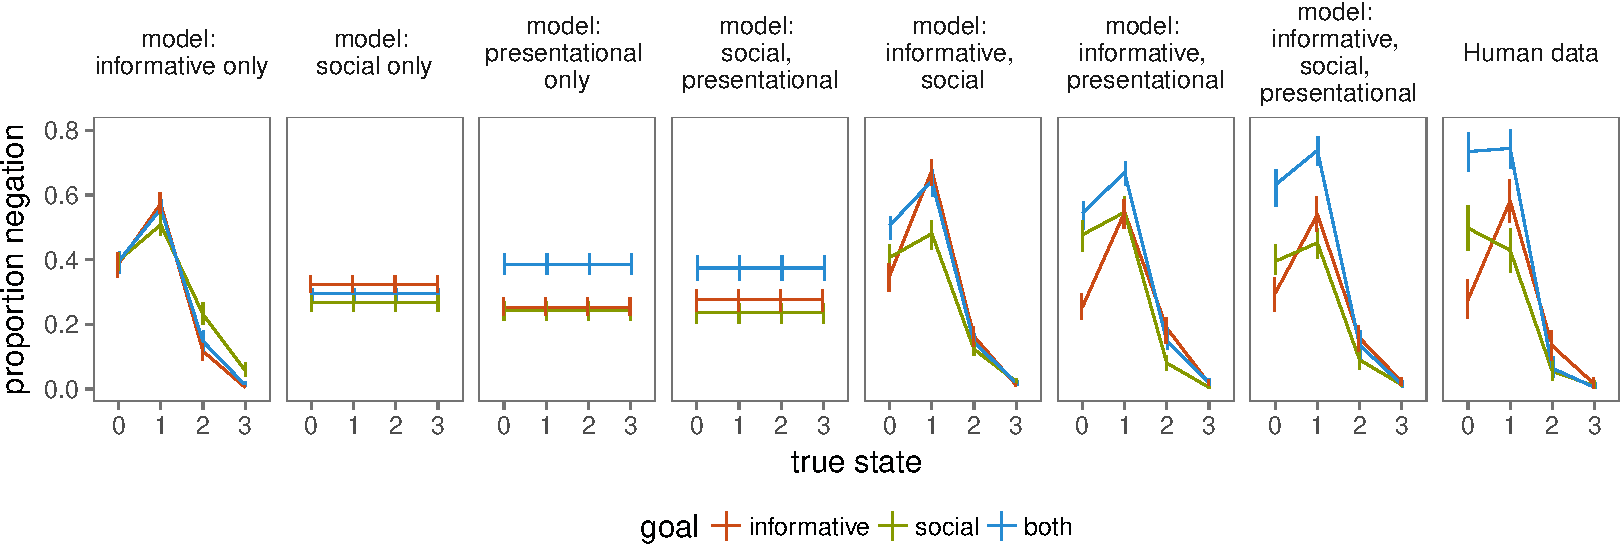
\includegraphics[width=\textwidth]{polite_manuscript_files/figure-latex/negation-1} \caption{Experimental results (left) and fitted model predictions (right) for average proportion of negation produced among all utterances, given true states (x-axis) and goals (colors).}\label{fig:negation}
\end{figure}


%References \textit{(4-10)}


% For your review copy (i.e., the file you initially send in for
% evaluation), you can use the {figure} environment and the
% \includegraphics command to stream your figures into the text, placing
% all figures at the end.  For the final, revised manuscript for
% acceptance and production, however, PostScript or other graphics
% should not be streamed into your compliled file.  Instead, set
% captions as simple paragraphs (with a \noindent tag), setting them
% off from the rest of the text with a \clearpage as shown  below, and
% submit figures as separate files according to the Art Department's
% instructions.


%\clearpage
%
%\noindent {\bf Fig. 1.} Please do not use figure environments to set
%up your figures in the final (post-peer-review) draft, do not include graphics in your
%source code, and do not cite figures in the text using \LaTeX\
%\verb+\ref+ commands.  Instead, simply refer to the figure numbers in
%the text per {\it Science\/} style, and include the list of captions at
%the end of the document, coded as ordinary paragraphs as shown in the
%\texttt{scifile.tex} template file.  Your actual figure files should
%be submitted separately.

\end{document}




















